\documentclass[11pt]{article}
\usepackage[utf8]{inputenc}
\usepackage{geometry}
\usepackage{graphicx}
\geometry{
	a4paper,
	total={165mm,242mm},
	inner=25mm,
	top=20mm,
}
\usepackage{hyperref}
\usepackage{enumitem}
\setitemize{itemsep=0pt}

\title{{\small \emph{a short guide to}\\}
\textsc{CMlib} -- Cell mapping algorithms in \texttt{C++}}
\author{Gergely Gyebrószki$^1$ \\
\emph{PhD candidate, research assistant} \\
$^1$: Dept. of Applied Mechanics, Budapest University of Technology and Economics
}
\date{27. February, 2019}

\begin{document}
\maketitle

{\small The latest version of this document is available at: \href{https://github.com/Gyebro/cell-mapping/blob/master/docs/tex/cell-mapping-cpp.pdf}{github.com/Gyebro/cell-mapping}}
	
\section{Introduction and goals}

\textsc{CMlib} is a library of cell mapping algorithms and utility functions and classes written in \texttt{c++}. 
Cell mapping methods are suitable for the global analysis of dynamical systems, they can be used to efficiently find state space objects (fixed points, periodic orbits and their corresponding domains of attractions) in a given discretized state space domain.\\
The goal of the \textsc{CMlib} library is to provide simple and efficient implementations of basic cell mapping algorithms allowing users to quickly utilize them to their problems or to integrate them into other applications independently of the underlying data types or differential equation solvers. To achieve this, \textsc{CMlib} mostly provides template base classes for various components, from which application-specific classes can derived.

% TODO: Intended audience, typical usage?

\section{Features}

\begin{itemize}
	\item Current version includes Simple Cell Mapping (SCM) and Clustered SCM methods, Generalized Cell Mapping (GCM) will be added.
	\item Entirely written in \texttt{c++} considering modern language features, with care to code clarity and documentation.
	\item Contains cross-platform and efficient implementations of cell mapping algorithms.
	\item Template approach allows replacing certain components (e.g. underlying data types, methods for state space discretization, used solvers) easily and independently from each other.
	\item Open source (with MIT licence), hosted on GitHub.
	\item Actively maintained and developed.
\end{itemize}


\section{Documentation}

The \textsc{CMlib} library is hosted on GitHub at: \href{https://github.com/Gyebro/cell-mapping}{github.com/Gyebro/cell-mapping}.\\
Doxygen generated code documentation (description of classes, APIs) can be found at the GitHub page of the repository: \href{https://gyebro.github.io/cell-mapping}{gyebro.github.io/cell-mapping}.\\
The latest version of this guide is available in the  \href{https://github.com/Gyebro/cell-mapping/blob/master/docs/tex/cell-mapping-cpp.pdf}{cell-mapping/docs} folder of the repository.
The repository's main page contains information about the currently developed features which can usually be found on development branches.

\section{Installation}

\subsection{Requirements}

The \textsc{CMlib} library can be used as a stand-alone \texttt{c++} library built from sources contained in the \texttt{cpp/cm} folder of the repository. The only requirement is a modern compiler which supports \texttt{c++11}.\\

For convenience and to aid cross-platform compilation, a \texttt{CMake} project is provided, and it is recommended to compile the library (and demonstrations) using \texttt{CMake} (available at \href{https://cmake.org/}{cmake.org}.) 
Alternatively, one can use an Integrate Development environment which can handle \texttt{CMake} projects, such as JetBrains CLion (which is available for free to university students and faculty at \href{https://www.jetbrains.com/clion/}{jetbrains.com/clion}).


\section{Examples}

\subsection{Simple pendulum}

\begin{figure}[h]
	\centering
	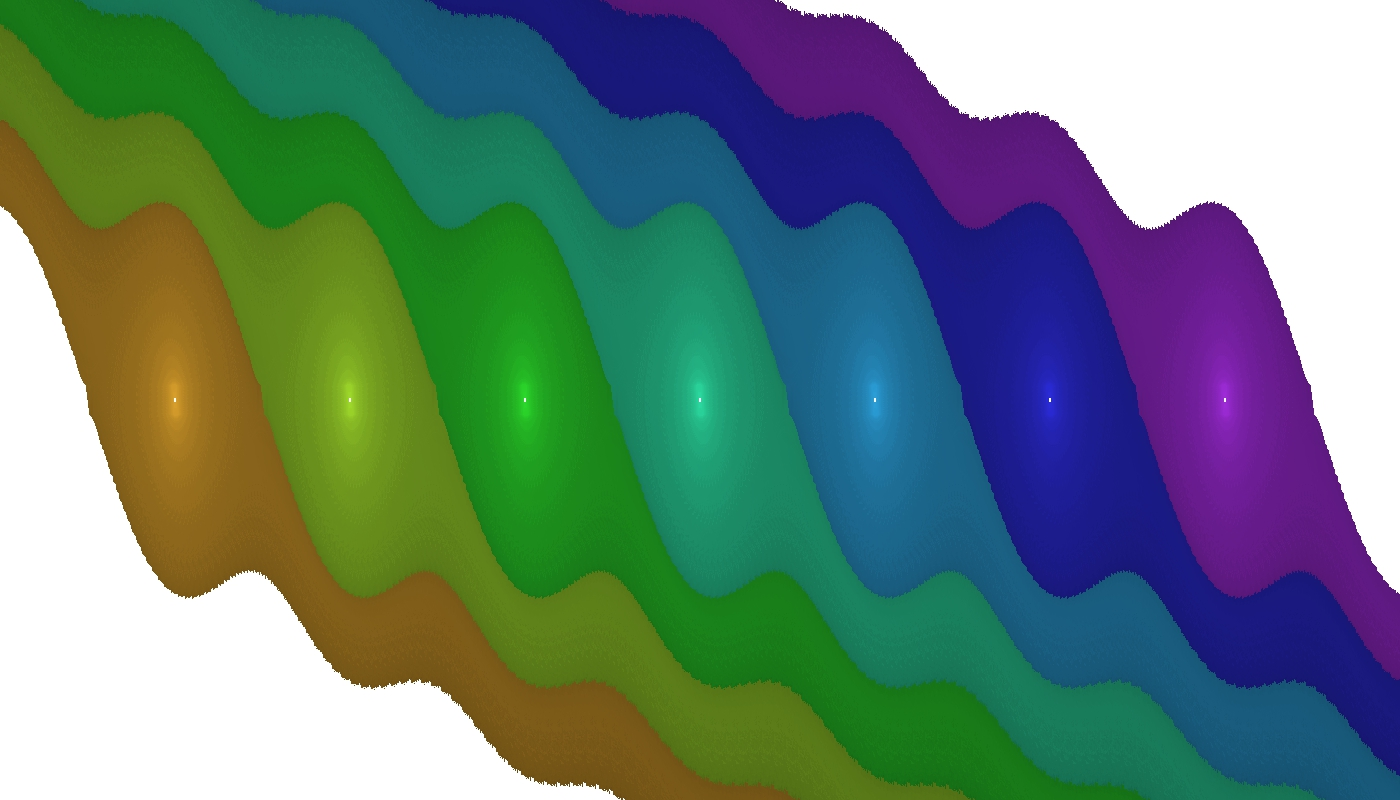
\includegraphics[width=12cm]{fig/pendulum.jpg}
	\caption{SCM results for the simple pendulum.}
\end{figure}


\subsection{Micro-chaos map}

\begin{figure}[h]
	\centering
	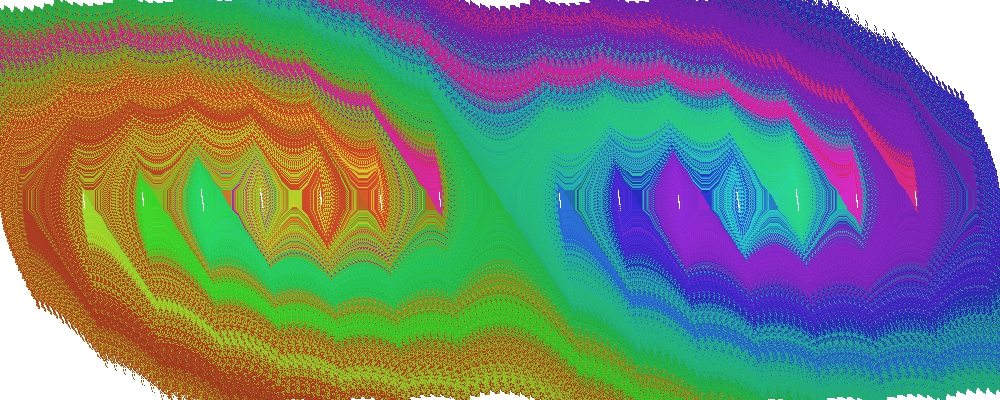
\includegraphics[width=12cm]{fig/microchaos.jpg}
	\caption{SCM results for the micro-chaos map.}
\end{figure}

\subsection{Duffing oscillator}

\begin{figure}[h]
	\centering
	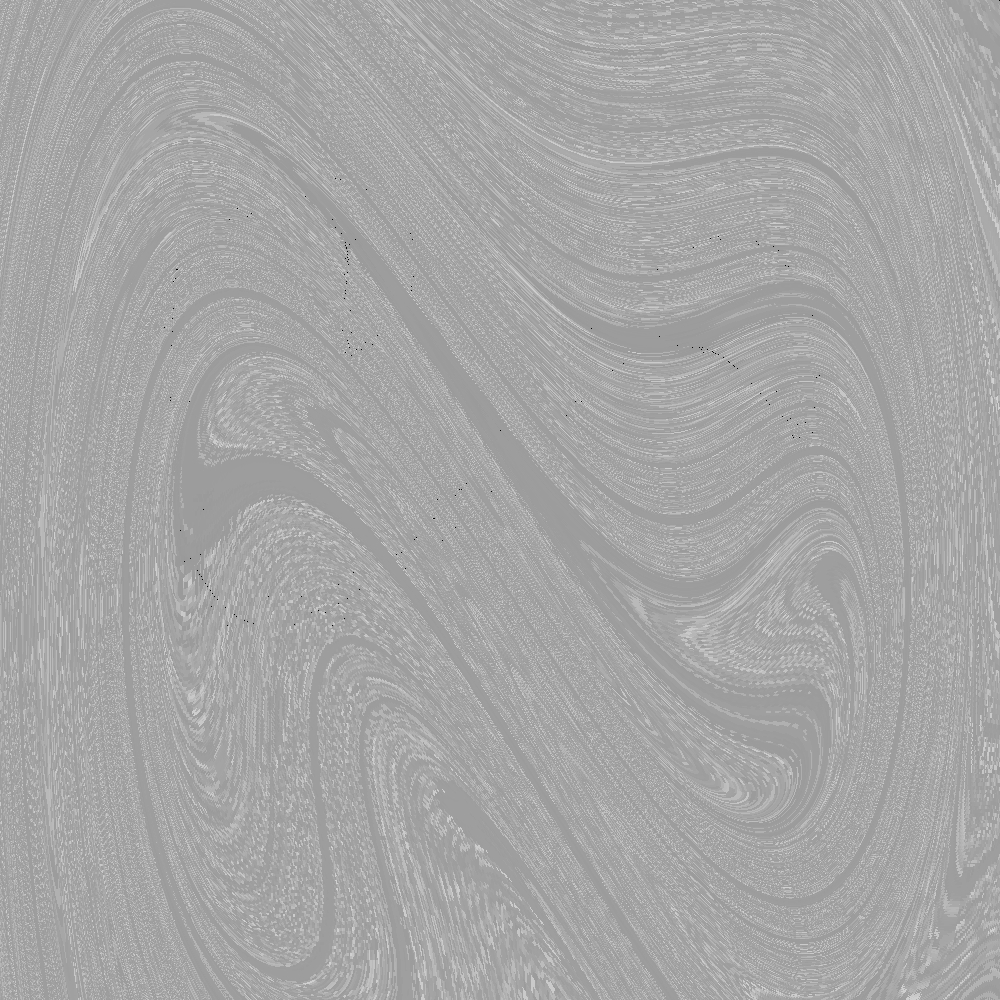
\includegraphics[width=10cm]{fig/duffing.jpg}
	\caption{SCM results for the Duffing oscillator Poincaré-section.}
\end{figure}

\end{document}